%%% PREAMBLE
\documentclass[12pt, a4paper]{article}
%% Packages
% Layout
\usepackage{parskip} % Changes parskip from being indent-based to adding vertical space
\usepackage[margin=2.5cm]{geometry} % Adjust margins to comply with 2,5cm standard
\usepackage{float}
\usepackage{pdflscape}

% Font management (for math and normal text)
\usepackage{sourcesanspro} % Changes font to Source Sans Pro
\usepackage{amssymb, amsmath, amsthm} % Adds math functionality, fonts and environments

% Bibliography and comment management
\usepackage[backend=biber,style=nature]{biblatex} % Bibliography management
\addbibresource{bibliography.bib} % Sets the bibliography-file
\usepackage{csquotes} % Adds babel-biliography compatability
\usepackage{comment} % Comments package for citation-purposes

% Appendix, attachments management
\usepackage[toc,page]{appendix} %
\renewcommand{\appendixtocname}{Appendiks}
\renewcommand{\appendixpagename}{\centering{Appendiks}}
\usepackage{pdfpages} % Including PDF-pages
    \usepackage{eso-pic}
    \usepackage{atbegshi}
    \usepackage{ifthen}
    \usepackage{calc}

% miscellaneous
\usepackage[danish]{translator}
\usepackage[danish]{babel} % Multi-lingual support - danish
\usepackage{lipsum} % Adds lipsum functionality
\usepackage{graphicx} %Titlepage - graphic support
\usepackage[colorlinks = true,linkcolor = blue,urlcolor  = blue,citecolor = blue,anchorcolor = blue]{hyperref} %Titlepage - customizes hyperlinks


%%% Document management
\begin{document}
%% Front matter
    \pagenumbering{roman}
    \begin{titlepage}
    \centering

    \vspace*{1cm}

    % Title and subtitle are enclosed between two rules.
    \rule{\textwidth}{1pt}

    % Title
    \vspace{.7\baselineskip}
    {\huge \textbf{Projekt 1 - Krisen kradser}}

    % Subtitle
    \vspace*{.5cm}
    {\LARGE Efterårssemester 2024}
    
    \rule{\textwidth}{1pt}

    \vspace{1cm}

    % Set this size for the remaining titlepage.
    \large

    % Authors side by side, using two minipages as a trick.

    \begin{table}[h]
        \centering
        \begin{tabular}{cc}
            \begin{minipage}{.5\textwidth}
                \centering
                Jeppe Bøgeskov Bech \\
                {\normalsize \url{jepp9920@zbc.dk}}
            \end{minipage}
            &
            \begin{minipage}{.5\textwidth}
                \centering
                Alexander Schade Knudsen \\
                {\normalsize \url{alex245h@zbc.dk}}
            \end{minipage} 
        \end{tabular}
        
        \vspace{1cm} % Adds vertical space between the rows
    
        \begin{minipage}{.5\textwidth}
            \centering
            Andreas Jensen \\
            {\normalsize \url{andr328q@zbc.dk}}
        \end{minipage}
    \end{table}
    





    

    % More authors can be inserted here with additional minipages.

    \vspace{1cm}

    % Report logo.
    
\includegraphics[width=.7\textwidth]{./assets/zbc_logo_black.jpg}

    \vfill

    % University and date information at the bottom of the titlepage.
    2. x \\
    ZBC Handels- og Teknisk gymnasium Slagelse \\
    Akademisk år 2024-2025 \\
    \today
\end{titlepage}
    \newpage
%    \input{preface/preface.tex}
    \section{Abstract}
This report encompasses the project of developing an application that can be used to manage crises. The application will be developed by a new company called "KEP". 
The application will be developed using a modern application development solution, ensuring optimal performance and compatibility.

\newpage
    \tableofcontents
    \newpage
%% Main body
    \pagenumbering{arabic}
    \section{Forord}
Vi vil gerne rette en tak til Morten Bach Jensen, agronom. Morten hjalp os med vores afgrødeberegner, han hjalp os også med information om sæddosering samt arealallokering, anvendt til beregning.

Vi vil endvidere rette en tak til Jacob Søgaard, Ph.d Video Quality Assessment, som har hjulpet os  \newpage % forord
    \section{Projektstyring}
\subsection{Rollefordeling}
\begin{table}[H]
  \centering
\begin{tabular}{l|l}
           & Roller:                                                \\ \hline
Alexander: & Visionsansvarlig, dokumentarist, strukturering         \\ \hline
Andreas:   & Konceptartist, informationssøgning                     \\ \hline
Jeppe:     & Produktansvarlig, programmør, artistsupervisor, vision
\end{tabular}
\caption{Viser rollefordelingen for vores projekt.}
\end{table}
\subsection{Tidsplan}
Vores tidsplan er håndteret via GitHubs indbygget funktion, se forneden, dog er den opdateret version her:
\begin{figure}[H]
  \centering
  \fbox{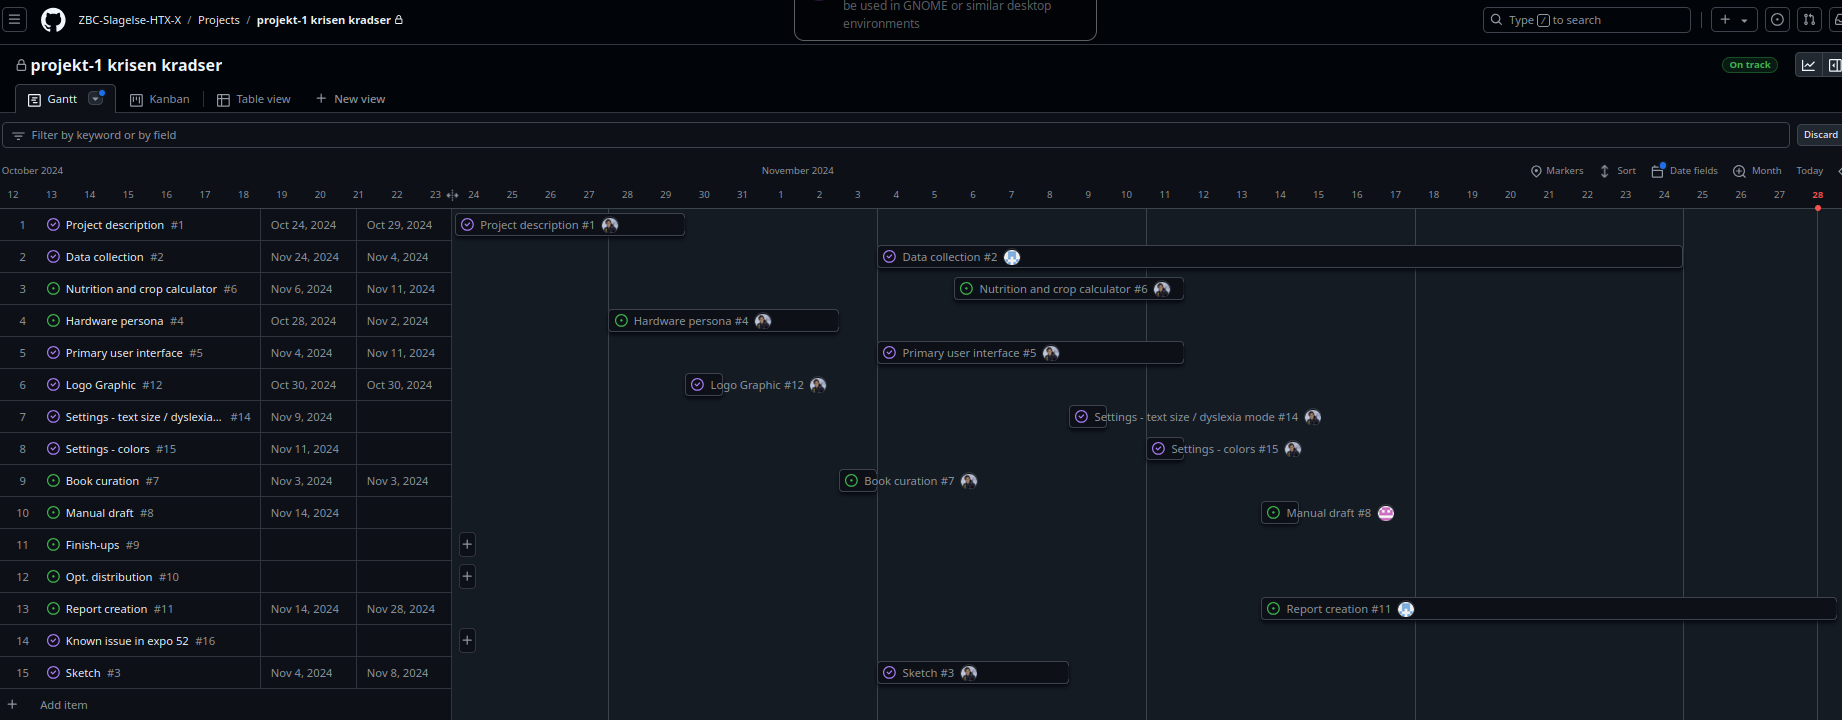
\includegraphics[width=\textwidth]{assets/section_2/2024-11-28_14-25.png}}
\end{figure}

Link til aktuel tidsstyring:
\subsection{Projektmappe}
Link: \href{https://github.com/ZBC-Slagelse-HTX-X/teknologiprojekt-1---Krisen-kradser/tree/main}{Vores GitHub fil}
 \newpage % 
    \section{Problemidentifikation}
\subsection{Idegenerering}
\subsubsection{Mindmap}
Vi har valgt at lave et mindmap, da dette er en effektiv måde at generere ideer på, og få et overblik over hvilke emner der er relevante at beskæftige sig med.
\begin{figure}[H]
    \centering
    \fbox{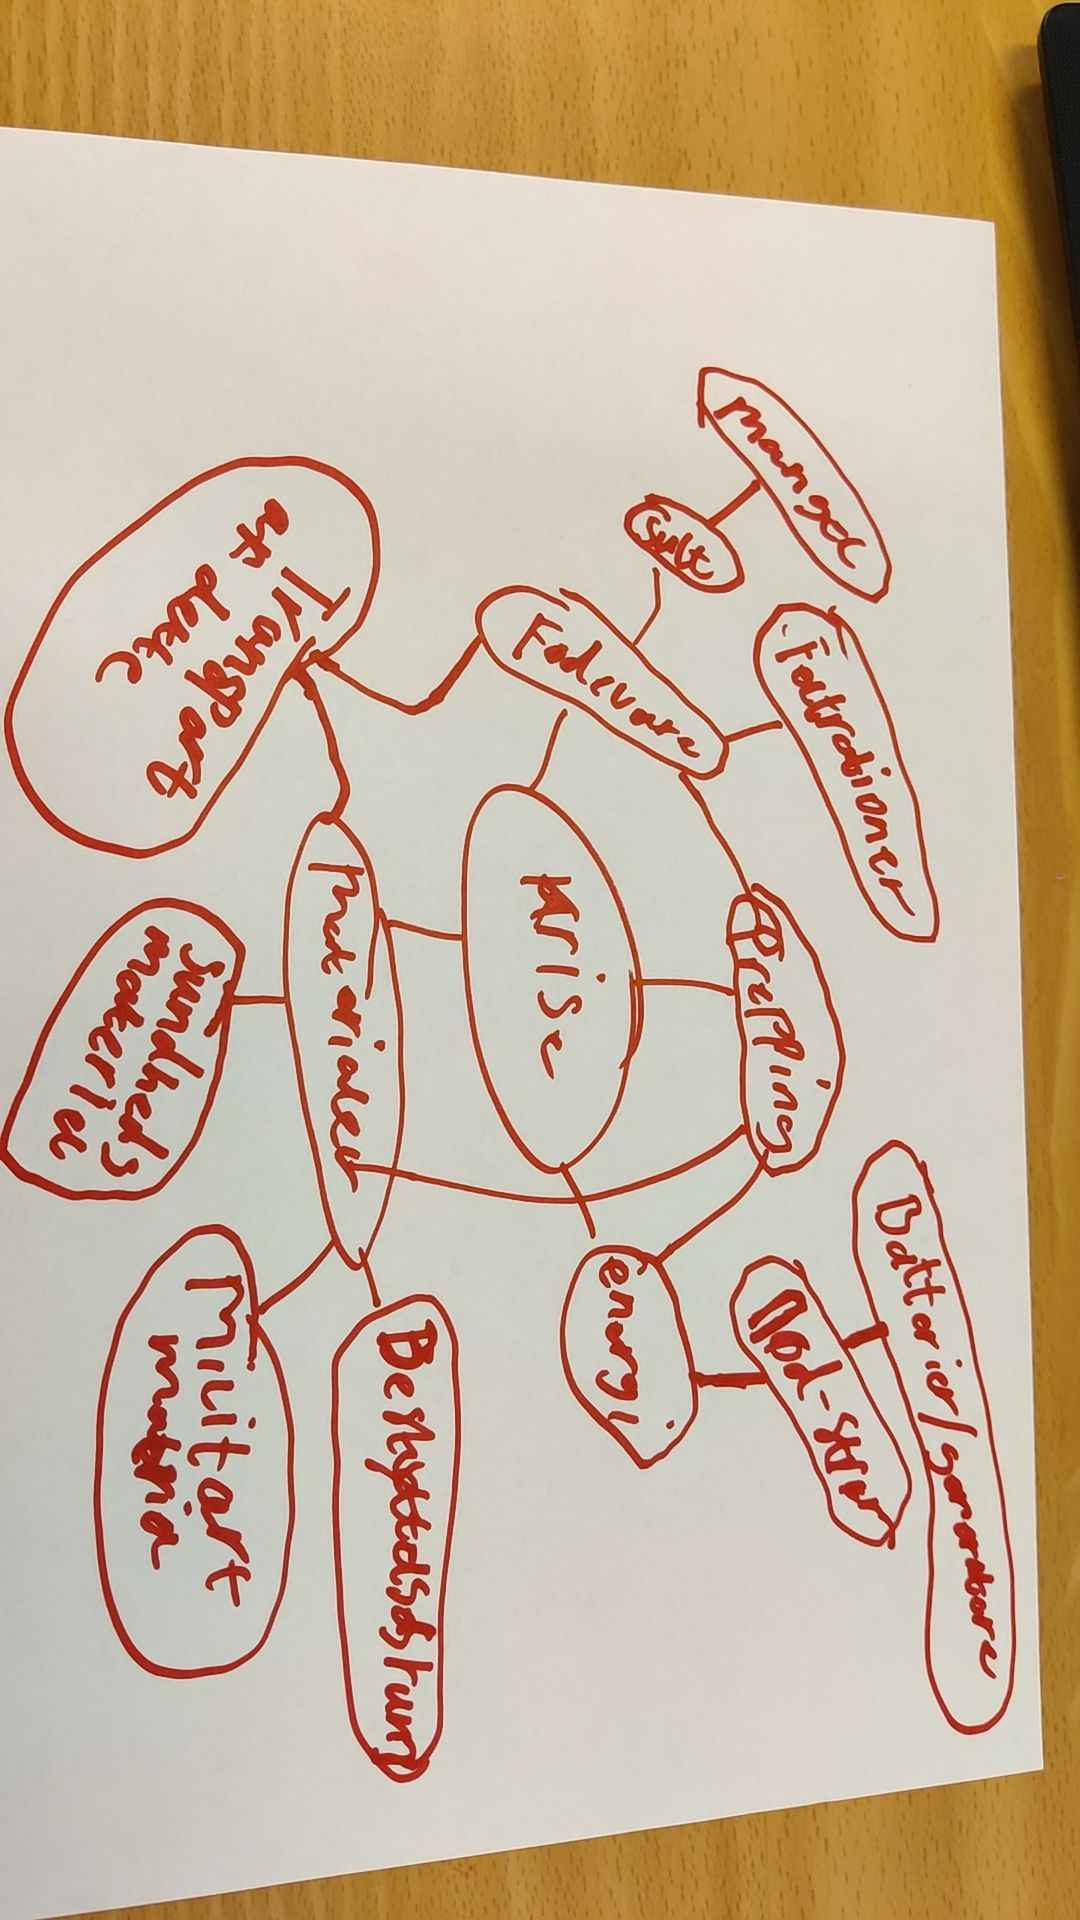
\includegraphics[scale=0.25, angle=90]{assets/section_3/mindmap.jpg}}
    \caption{Viser vores mindmap}
\end{figure}

\subsubsection{Lyskurven}
Lyskurven er en metode, man kan bruge til at sortere ideerne i forhold til hvilke der er mest relevante.
----- Bla bla waffel mere on lyskurvediagrammet -----

\begin{table}[H]
    \centering
    \begin{tabular}{|c|c|c|}
        \hline
        Fødevarer & \textbf{Grøn} \\
        \hline
        Beskyttelsesrum & \textbf{Gul} \\
        \hline
        Nødstrøm & \textbf{Rød} \\
        \hline
    \end{tabular}
    \caption{Viser et meget abstrakt lyskurvediagram i form af en tabel; det vi anvendte}
\end{table}

\subsubsection{Identificering af nøgleproblem}
Ved identifikation af et nøgleproblem, kan man sortere i sine ideer ved at opstille følgende spørgsmål:
\begin{enumerate}
    \item Hvorfor er det her interessant?
    \item Hvem er det interessant for?
    \item Er det noget, vi laver for vores egen fornøjelses skyld?
    \item Er det noget, som en bestemt gruppe i samfundet kan have gavn af, eller er det noget, der er til gavn for alle?
\end{enumerate}
** Spørsmålene som vi her gør brug af er hentet fra systimebogen\footnote{\href{https://projektarbejdet.systime.dk/?id=271}{Projektarbejdet}}

Besvarelsen på disse spørgsmål ser således ud:
\begin{enumerate}
    \item Krisehåndtering er et interessant emne, da det har en stor betydning for alle i samfundet.
    \item Det er relavant for alle.
    \item Nej, ideen med produktet er at kunne hjælpe almindelige mennesker med at håndtere kriser, mindre som store.
    \item Produktet skulle kunne gavne alle, som kunne stå i en krisesituation.
\end{enumerate}

Vi kan nu se, at det mest interessante emne er krisehåndtering, da det har en så stor relavans for grupper i samfundet, og det er noget som vi ser der er behov for. \newpage
    \input{section}
    \newpage
%% Back matter
     \printbibliography[heading=bibintoc,title={Litteraturliste}]
     \begin{appendices} \newpage
         \section{Projektbeskrivelse \label{appendiks-projektbeskrivels}} \newpage
        \renewcommand*{\thepage}{A\arabic{page}}
         %
\includepdf[pages=-,delta=5 5,frame=true,landscape=true,nup=1x2,pagecommand={\thispagestyle{plain}}]{./project description/project_description.pdf}
%         \renewcommand*{\thepage}{\arabic{page}}
%         \section{Logbog} \newpage
%         \renewcommand*{\thepage}{B\arabic{page}}
%         \includepdf[pages=-,delta=5 5,frame=true,landscape=true,nup=1x2,pagecommand={\thispagestyle{plain}}]{Log/log.pdf}
%         \renewcommand*{\thepage}{\arabic{page}}
     \end{appendices}
  \end{document}
